\chapter{Introducción}
\label{cap:capitulo1}
\setcounter{page}{1}

\begin{flushright}
\begin{minipage}[]{10cm}
\emph{La automatización no es el enemigo del trabajador, sino la clave para su evolución}\\
\end{minipage}\\
\end{flushright}

\vspace{1cm}

La automatización ha sido un pilar fundamental en el desarrollo de la industria moderna, permitiendo mejoras significativas en eficiencia, calidad y seguridad. Desde la evolución Industrial hasta la actualidad, la evolución de las tecnologías ha dado paso a sistemas cada vez más sofisticados, donde la integración de robots ha transformado los entornos de producción, ofreciendo resultados de mayor calidad y reduciendo costes y tiempos de producción. En particular, la robótica industrial ha desempeñado un papel clave en sectores como la automoción, la electrónica y la manufactura, ofreciendo soluciones flexibles y altamente eficientes para la producción en serie.\\

En este capítulo se presentará el contexto en el que se desarrolla este trabajo, proporcionando una visión general de la automatización en la industria y su evolución hasta la actualidad. Posteriormente, se acotará el enfoque hacia la robótica industrial, destacando su impacto en la optimización de procesos productivos. Finalmente, se delimitará el ámbito específico de este estudio, centrado en la automatización de una línea de producción robotizada, analizando sus beneficios, retos y las tecnologías empleadas.

\section{La automatización industrial}
\label{sec:primeraseccion} % etiqueta para luego referenciar esta sección

\subsection{Conceptos básicos de la automatización industrial}

La automatización industrial consiste en la implementación de sistemas de control, como computadoras, controladores lógicos programables (PLCs), robots y tecnologías de la información, para gestionar maquinaria y procesos productivos en el sector industrial \cite{definicion}. Su propósito principal es reducir la intervención humana, reemplazando tareas manuales, especialmente aquellas que implican riesgos, por procesos automatizados .

Este concepto surge como una evolución de la mecanización industrial, incorporando dispositivos con gran capacidad de control para optimizar la eficiencia en la fabricación. Con los avances tecnológicos y la llegada de la Industria 4.0, las empresas están modernizando sus sistemas de producción mediante el uso de control informatizado, lo que les permite mejorar la precisión, calidad y rendimiento de sus operaciones \cite{definicion}. \\

El término ``automatización'' tiene su origen en las palabras griegas ``auto'' (por sí mismo) y ``matos'' (movimiento), y se aplica a mecanismos capaces de funcionar de manera autónoma. Los sistemas automatizados ofrecen un rendimiento superior a los manuales en términos de precisión, potencia y velocidad. En el ámbito del control industrial, es posible monitorizar y regular simultáneamente diversas variables de proceso, como temperatura, flujo, presión, distancia y niveles de líquido, mediante el uso de PLCs (computadora industrial la cual graba la información de las entradas en memoria, las procesa y escribe en las salidas las acciones oportunas), PACs (Controladores Automatizados Programables que integran PLC y PC), o PCs. \cite{definicion}. \\

La estructura de un sistema de automatización industrial se puede representar mediante un triángulo jerárquico de cinco niveles:

\begin{enumerate}
    \item \textbf{Nivel de gestión}: La alta gerencia usa sistemas ERP para controlar y monitorear todos los procesos de la empresa, desde la producción hasta ventas, compras y proyectos, asegurando eficiencia y alineación entre equipos.\cite{niveles_automatizacion_2}.
    \item \textbf{Nivel de operación}: Este nivel está controlado por el sistema MES (Un sistema MES conecta el mundo digital con la producción, permitiendo supervisar y sincronizar cada fase del proceso \footnote{  (N.d.). Cursosaula21.com. Retrieved April 7, 2025, from \url{ https://www.cursosaula21.com/que-es-un-sistema-mes/}}), para monitorear la producción. Este sistema integra datos de operaciones, mantenimiento, seguridad, logística y calidad, permitiendo a la gerencia tomar decisiones informadas sobre todo el proceso, desde las materias primas hasta el producto final. \cite{niveles_automatizacion_2}.
    \item \textbf{Nivel supervisor}: Compuesto por un ordenador industrial que utiliza software especializado para el control de procesos. Su principal objetivo es la parametrización y visualización del proceso y suele utilizars el protocolo de de comunicación Ethernet industrial \cite{niveles_automatizacion_1}.
    \item \textbf{Nivel de control}: Incluye dispositivos como PLCs que ejecutan las órdenes del nivel supervisor y controlan directamente la maquinaria en tiempo real. Estos pueden estar conectados a varios dispositivos de E/S y se comunican mediante protocolos industriales \cite{niveles_automatizacion_1}.
    \item \textbf{Nivel de campo}: Constituido por sensores y actuadores que interactúan directamente con el proceso físico conectados al PLC a través de un bus de campo. Los actuadores ejecutan acciones según las instrucciones recibidas normalmente a través de una conexión punto a punto con el PLC. \cite{niveles_automatizacion_1}. 
\end{enumerate}

Esta estructura permite una gestión eficiente y organizada de los procesos industriales, asegurando que cada componente funcione de manera integrada para optimizar la producción. 

\begin{figure} [h!]
  \begin{center}
    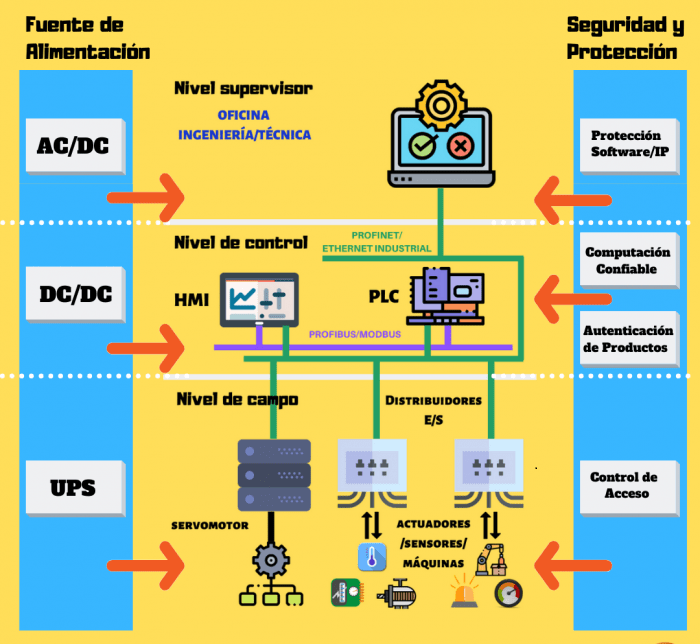
\includegraphics[width=16cm]{figs/esquema_automatizacion}
  \end{center}
  \caption{\centering Niveles de la pirámide de automatización. (no conisigo poner la refernecia en el titulo de la imagen)}  
  \label{fig:esquema_automatizacion}
\end{figure}  

% \footnote{ La Pirámide De Automatización: Clave Para La Integración De Sistemas En Plantas Industriales - Omnielectric Web. (2024, July 2). Omnielectric. \url{ https://omnielectric.es/piramide-de-automatizacion/}}


\subsection{Tipos de automatización industrial}

Los sistemas de automatización industrial se clasifican principalmente en cuatro tipos según su nivel de flexibilidad y aplicación en los procesos productivos:

\begin{enumerate}
    \item \textbf{Automatización fija}: Utilizada en procesos específicos y repetitivos donde no se requieren modificaciones en el diseño del producto debido a que aplicar modificaciones resulta casi imposible. Es ideal para la producción a gran escala de productos estables \cite{tipos_industrial}.
    \item \textbf{Automatización programable}: Aplicada en la fabricación por lotes, permite modificar el proceso mediante reprogramación, aunque esto puede consumir tiempo \cite{tipos_industrial}.
    \item \textbf{Automatización flexible}: Variante más avanzada de la automatización programable, que facilita cambios rápidos y automáticos en la producción sin interrupciones significativas \cite{tipos_industrial}.
    \item \textbf{Sistema Integrado de Automatización}: Conjunto de máquinas, procesos y datos sincronizados bajo un único sistema de control. Integra herramientas como CAD, CAM, robots y sistemas de transporte automatizados para optimizar la producción \cite{tipos_industrial}.
\end{enumerate}

\subsection{Ventajas y desventajas de la Automatización Industrial}

La automatización industrial ha transformado profundamente los procesos de producción, introduciendo tecnologías avanzadas que permiten aumentar la eficiencia, mejorar la calidad y reducir los costos operativos. Sin embargo, junto con estos beneficios, también surgen desafíos y limitaciones que deben ser considerados por las empresas antes de implementar estos sistemas. A continuación, se presentan las principales ventajas y desventajas de la automatización industrial:

\begin{itemize}

 \item \textbf{Mayor productividad laboral}: La automatización acelera los procesos de producción, permitiendo fabricar más productos con una mejor calidad. Las nuevas tecnologías pueden operar de manera continua sin perder precisión, lo que incrementa la eficiencia y el rendimiento por hora de trabajo  \cite{des_ventajas_1}.

 \item \textbf{Mejora en la calidad del producto}: Uno de los principales beneficios de la automatización es la reducción de la cantidad de unidades defectuosas. Los sistemas automatizados garantizan una mayor uniformidad y precisión en la fabricación, cumpliendo con los estándares de calidad \cite{des_ventajas_2}.
   
\item \textbf{Reducción de costos de producción}: La automatización permite disminuir el gasto en mano de obra al reemplazar tareas repetitivas con maquinaria, lo que reduce el costo unitario de producción. Los sistemas automatizados operan de manera constante, aumentando la eficiencia y proporcionando un alto retorno de inversión al minimizar costos laborales, ausencias y otros gastos operativos \cite{des_ventajas_1}.

\item \textbf{Menos trabajo manual repetitivo}: En muchas industrias, es necesario supervisar constantemente variables como temperatura, presión o nivel de líquidos. Un sistema automatizado permite gestionar estas tareas mediante controladores de lazo cerrado, reduciendo la necesidad de intervención humana en actividades rutinarias \cite{des_ventajas_1}.

\item \textbf{Mayor seguridad}: Al implementar un sistema automatizado, los trabajadores pasan de realizar tareas directamente en el proceso a supervisarlas, lo que disminuye los riesgos laborales. Las máquinas pueden operar en entornos peligrosos o extremos, sustituyendo a los empleados en situaciones de alto riesgo, reduciendo así los accidentes laborales \cite{des_ventajas_2}.

\item \textbf{Facilita la monitorización remota}: Muchas operaciones industriales requieren ser controladas a distancia para una supervisión más eficiente. Los sistemas automatizados permiten la comunicación entre el área de producción y el centro de control, permitiendo a los operadores gestionar los procesos de manera remota \cite{des_ventajas_2}.

\item \textbf{Aumento de la contaminación}: Muchas máquinas requieren motores que funcionan con combustibles o productos químicos que pueden generar emisiones contaminantes \cite{des_ventajas_1}.

\item \textbf{Menor flexibilidad}: Una máquina automatizada está diseñada para realizar tareas específicas, lo que limita la capacidad de adaptación a nuevas funciones en comparación con un trabajador humano. Actualmente, ciertas tareas, como el ensamblaje de productos con formas irregulares, siguen dependiendo del trabajo manual \cite{des_ventajas_1}.

\item \textbf{Altos costos de implementación}: La inversión inicial para adoptar un sistema automatizado es elevada. Además de los gastos en investigación y desarrollo, es necesario considerar los costos de mantenimiento, formación del personal y servicio técnico, lo que suma un desafío económico para las empresas que buscan automatizar sus procesos \cite{des_ventajas_2}.
\end{itemize}

\begin{figure} [h!]
  \begin{center}
    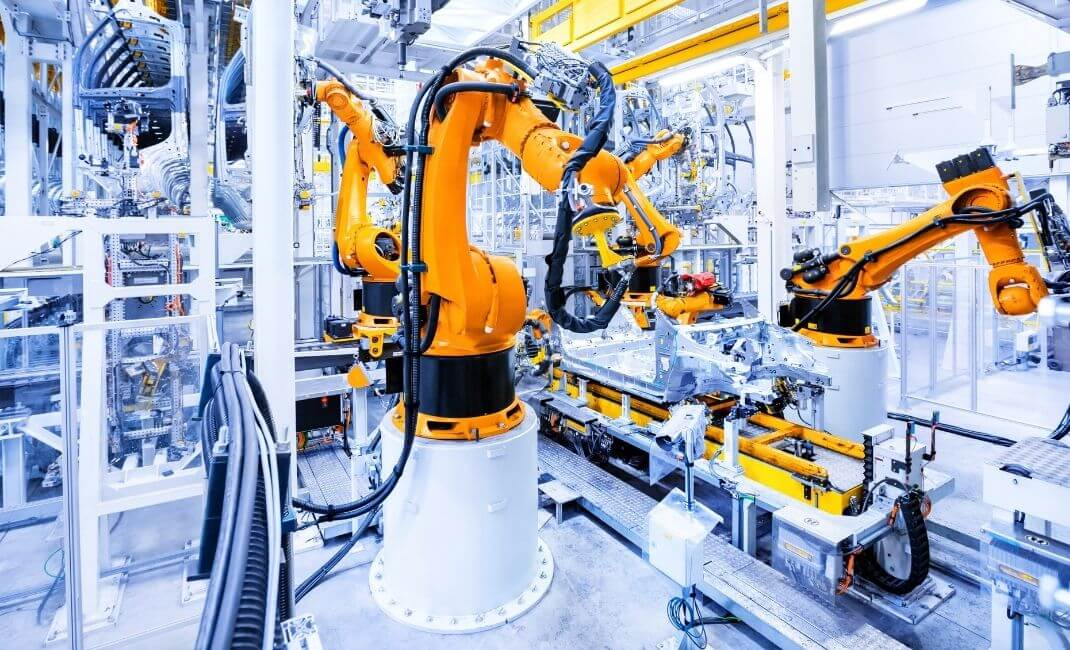
\includegraphics[width=13cm]{figs/automatizacion_industrial.jpg}
  \end{center}
  \caption{\centering Ejemplo de aplicación de automatización industrial.}
  \label{fig:automatizacion_industrial}
\end{figure}

\section{La robótica}
\label{sec:segundaseccion} % etiqueta para luego referenciar esta sección

La robótica es la disciplina científica que integra conocimientos de electrónica, mecánica e informática para desarrollar sistemas automatizados capaces de realizar tareas de manera autónoma o semiautónoma. Los componentes que conforman un robot son esenciales para su funcionamiento, desde la estructura mecánica (brazos, ruedas, actuadores, etc.), que debe garantizar un movimiento preciso y estabilidad, hasta los sistemas electrónicos que deben ser totalmente compatibles y funcionales para permitir la correcta operación. Además, los algoritmos que se implementan deben ser robustos, seguros y capaces de adaptarse a diversas situaciones y condiciones del entorno.

Entre estos componentes, uno de los más importantes para lograr dicha adaptación al entorno son los sensores, ya que juegan un papel crucial proporcionando al robot la información necesaria sobre su entorno. Estos sensores, de diversos tipos, miden una amplia gama de magnitudes físicas, como la luz, posición, velocidad, fuerza, temperatura..., funcionando de manera análoga a los órganos sensoriales en los seres humanos. 

Una vez que los sensores recogen los datos del entorno, el software del robot procesa esta información, proporcionando la inteligencia necesaria para tomar decisiones. Utilizando algoritmos avanzados o inteligencia artificial, el robot es capaz de generar respuestas adecuadas a las entradas, lo que resulta en la ejecución de una acción específica, como un movimiento o la interacción con su entorno. 

Finalmente, los actuadores son los encargados de ejecutar las acciones determinadas por el sistema de control, permitiendo que el robot lleve a cabo tareas como moverse o manipular objetos. Los actuadores son fundamentales para la efectividad del robot, ya que son los elementos que materializan las decisiones procesadas en acciones físicas tangibles. 

\begin{figure} [h!]
  \begin{center}
    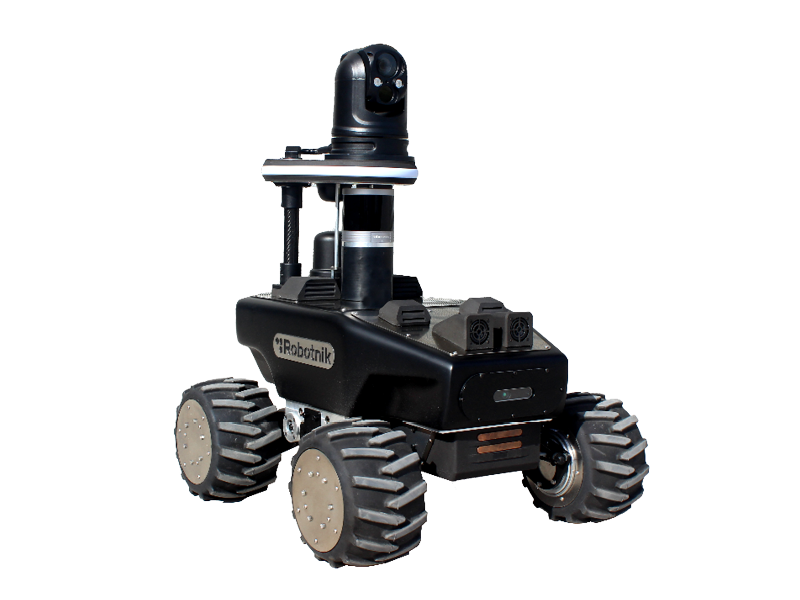
\includegraphics[width=10cm]{figs/Robot_intro}
  \end{center}
  \caption{\centering RB-WATCHER de Robotink.}
  \label{fig:Robot_intro}
\end{figure}

\subsection{Robótica Industrial}

Según la norma internacional ISO 8373:2012 un robot industrial se define como ``un manipulador multifuncional, reprogramable y controlado automáticamente, programable en tres o más ejes que puede estar fijo en un área o móvil para su uso en aplicaciones de automatización industrial'' \cite{definicion_iso}. Todo ello a partir de trayectorias variables para ejecutar diversas tareas cíclicas y adaptables. 

La robótica industrial es una disciplina de la ingeniería robótica dedicada al diseño, desarrollo y fabricación de robots industriales con el propósito de automatizar tareas repetitivas tradicionalmente realizadas por seres humanos. Estos sistemas robóticos se caracterizan por seguir una secuencia de instrucciones predefinidas, ejecutando ciclos de trabajo continuos en líneas de producción de diversos sectores industriales. Estos robots son considerados industriales debido a que se utilizan en la industria manufacturera en sectores como la automoción, electrónica, alimentación, farmacéutico... En ellos contribuyen significativamente a mejorar la eficiencia, la velocidad y la calidad de los procesos productivos \cite{info_robotica_industrial_1}. 

A diferencia de los robots de servicio, los robots industriales operan en entornos altamente controlados, lo que simplifica su programación y control. Debido a estas condiciones estables, estos robots suelen tener más de tres grados de libertad, permitiéndoles realizar movimientos complejos con gran precisión. Aunque su aplicación principal ha sido históricamente en entornos industriales, su uso se ha expandido hacia sectores como la minería, la agricultura, el comercio y la salud, demostrando su versatilidad y adaptabilidad. \\

Diferenciar entre brazo robotico y brazo industrial \\

Desde la aparición de los primeros prototipos de robots industriales, ha surgido un debate sobre su impacto en el empleo humano, con preocupaciones respecto a una posible sustitución de la mano de obra. Sin embargo, numerosos estudios sostienen que, lejos de desplazar a los trabajadores, estos sistemas robóticos buscan mejorar las condiciones laborales, eliminando tareas monótonas o peligrosas \cite{info_robotica_industrial_2}. 

\begin{figure} [h!]
  \begin{center}
    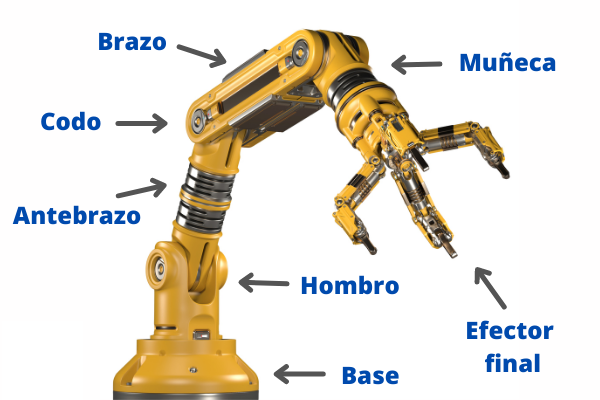
\includegraphics[width=9cm]{figs/brazo_industrial}
  \end{center}
  \caption{\centering Partes de un brazo robótico industrial.}
  \label{fig:brazo_industrials}
\end{figure}

\subsection{Tipos de robots industriales}
 
Existen una gran variedad de diseños y configuraciones de robots industriales debido a las diversas aplicaciones y entronos en los que estos se emplean. Esta clasificación puede realizarse según diversos criterios, siendo el más común el tipo de configuración mecánica, que determina los grados de libertad, el alcance y la versatilidad del robot.

\subsubsection{Robot cartesiano}

Los robots cartesianos se componen de tres articulaciones prismáticas y utilizan el sistema de coordenadas tridimensionales, el cual lo forman los ejes X, Y y Z. Los movimientos de estos robots son lineales por lo que su funcionamiento es sencillo y se limita a movimiento de traslación. Suelen ser utilizados para mover cargas pesadas linealmente en las que no es necesario rotarlas \cite{tipos_robots_1}. 

\begin{figure} [h!]
  \begin{center}
    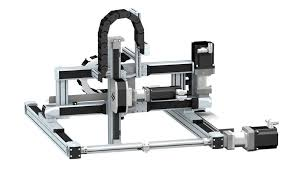
\includegraphics[width=7cm]{figs/robot_cartesiano}
  \end{center}
  \caption{\centering Robot cartesiano.}
  \label{fig:robot_cartesiano}
\end{figure} 

\subsubsection{Robot antropomórfico}

Estos robots articulados son los más comunes en el sector de fabricación enfocados en aplicaciones complejas como el montaje de productos, soldadura o mecanizado. El ``end effector'' (pieza situada en el extremo final del brazo) poseen seis grados de libertad para poder operar en cualquier situación. Los brazos de este estilo poseen tres articulaciones de giro y otra opcional en el EOAT (herramientas conectadas al extremo final del brazo con las cuales se opera con el entorno) \cite{tipos_robots_2}.

\begin{figure} [h!]
  \begin{center}
    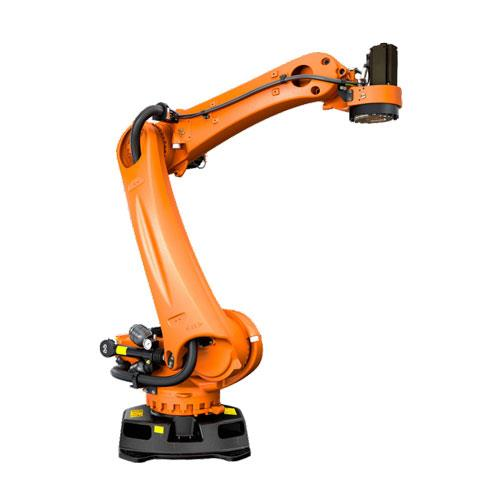
\includegraphics[width=6cm]{figs/robot_antropomorfico}
  \end{center}
  \caption{\centering Robot antropomórfico.}
  \label{fig:robot_antropomorfico}
\end{figure} 

\subsubsection{Robot cilíndrico}

Los robots cilíndricos se caratcerizan por tener movimientos cilíndricos debido a que están compuestos de dos articulaciones prismáticas y otra de revolución. Esta morfología le permite movimientos de rotación en torno a su propio eje y con las articulaciones prismáticas ajusta la altitud y radio de trabajo. Su principal aplicación es la de ``pick and place'' las cuales no requieren desplazamiento \cite{tipos_robots_2}.

\begin{figure} [h!]
  \begin{center}
    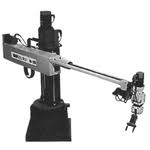
\includegraphics[width=5.5cm]{figs/robot_cilindrico}
  \end{center}
  \caption{\centering Robot cilíndrico.}
  \label{fig:robot_cilindrico}
\end{figure} 

\subsubsection{Robot SCARA}

Este tipo de robots tiene como peculiaridad que poseen un brazo con libertad en un plano XY, pero con restricción de movimiento en el eje Z. Estos modelos están formados por dos eslabones en adición a dos juntas de revolución y una prismática. La función de la articulación prismática es desplazar en el eje Z el EOAT y tiene diversas aplicaciones como la paletización, el ensambalaje o biomedicina \cite{tipos_robots_1}.

\begin{figure} [h!]
  \begin{center}
    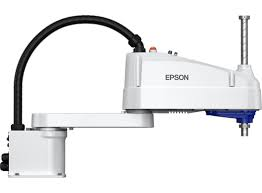
\includegraphics[width=6cm]{figs/robot_SCARA}
  \end{center}
  \caption{\centering Robot SCARA.}
  \label{fig:robot_SCARA}
\end{figure} 

\subsubsection{Robot delta}
Los robots delta están formados por tres eslabones unidos al un EOAT mediante tres juntas universales y una base común. La base está formada por tres articulaciones primáticas o en su lugar accionadas por revoluciones, y, su función, es proporionarle cuatro grados de libertad al EOAT para que pueda moverse en todos los ejes cartesianos y girar sobre su eje Z. Sus principales aplicaciones son la de ``pick and place'' de forma veloz (debido a que no tiene que mover toda la estructura mecánica como otro tipo de brazos, sino que solo mueve el TCP o punto central de la herramienta). en la industria alimentaria, electrónica y farmacéutica \cite{tipos_robots_2}.


\begin{figure} [h!]
  \begin{center}
    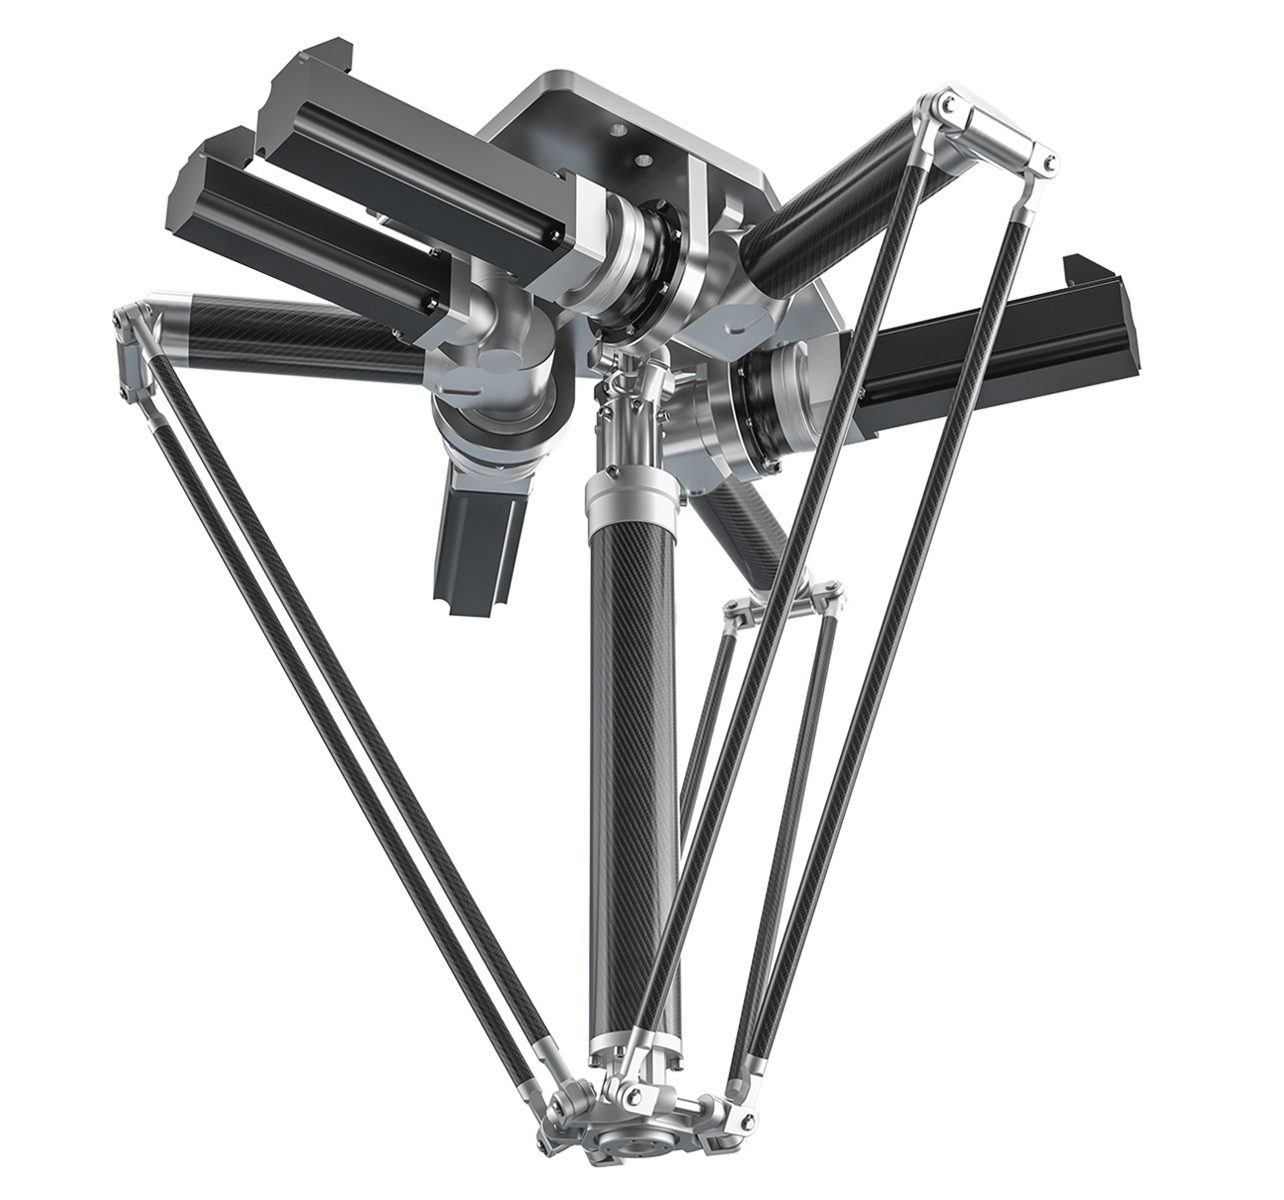
\includegraphics[width=5cm]{figs/robot_delta}
  \end{center}
  \caption{\centering Robot delta.}
  \label{fig:robot_delta}
\end{figure} 

\subsubsection{Robot esférico}

Estos robots también tienen el nombre de robots polares y están basados en el sistema de coordenadas polares consiguiendo un área de trabajo esférica. La longitud del enlace entre el EOAT y la articulación de revolución más cercana establecen su rango de movimiento permitiendo un mayor alcance en comparación a otros modelos. So aplicación más común es en aplicaciones de carga de mñaquinas debido a su largo alcance \cite{tipos_robots_2}.

\begin{figure} [h!]
  \begin{center}
    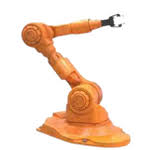
\includegraphics[width=4cm]{figs/robot_esferico}
  \end{center}
  \caption{\centering Robot esférico.}
  \label{fig:robot_esferico}
\end{figure} 

\subsubsection{Historia}

Entrando al siglo XXI se crean los primeros robots colaborativos, conocidos como cobots, concebidos para cooperar de manera directa con las personas. Estos dispositivos se caracterizan por su seguridad, adaptabilidad y facilidad de programación, convirtiéndose en una solución ideal para entornos industriales donde es necesario combinar tareas manuales y automatizadas. 

En los años 2010, la Industria 4.0 emergió como una nueva fase en la manufactura, caracterizada por la digitalización y la interconexión de sistemas de producción.  Los robots industriales se convirtieron en componentes clave de las fábricas inteligentes, colaborando estrechamente con humanos y otros sistemas automatizados para optimizar la eficiencia y la flexibilidad en la producción\footnote{Sutori. (n.d.). Sutori.com. Retrieved February 24, 2025, from \url{ https://www.sutori.com/es/historia/linea-de-tiempo-evolucion-de-la-robotica-industrial--6w6pytow1tj3grr5scVKU1Ns}}. 

\section{Unión entre la automatización y la robótica}
\label{sec:terceraseccion}

definicion PLC, comunicaciones, simulador didactico, guía Gemma, Grafcet \\

\section{Motivación del trabajo}
\label{sec:cuartaseccion}

A lo largo de mi formación académica, he adquirido conocimientos en diversas áreas de la robótica, incluyendo robótica de servicio, automatización, planificación, sistemas distribuidos y programación con Arduino, entre otras. Sin embargo, el ámbito que más ha despertado mi interés ha sido el de la robótica industrial. \\

Es cierto que la robótica industrial no tiene una presencia destacada en mi formación académica, ya que únicamente se imparten dos o tres asignaturas centradas en este ámbito. En consecuencia, mi conocimiento sobre el sector no es especialmente profundo. No obstante, desde el primer día me ha resultado un área fascinante, especialmente todo lo relacionado con los brazos robóticos y los PLCs, cuya programación es mucho más interactiva y dinámica en comparación con otros tipos de robots, como aquellos que emplean ROS. Además, me resulta especialmente atractivo trabajar en un entorno controlado, ya que ello me permite desarrollar programas con la certeza de que ningún factor externo afectará su funcionamiento. \\

Con este trabajo, mi objetivo es adquirir una formación sólida y obtener los conocimientos necesarios para desarrollarme profesionalmente en el sector de la robótica industrial, complementando y ampliando así lo aprendido durante la carrera. Considero que este ámbito tiene un gran futuro, ya que la producción industrial en masa seguirá siendo fundamental debido al consumismo global y al crecimiento demográfico. Además, el sector continúa evolucionando constantemente con el desarrollo de nuevas técnicas y robots, lo que ha impulsado su expansión desde sus inicios en la década de 1940. He elegido esta rama de la robótica porque es la que más me apasiona y me genera mayor satisfacción entre todas las que he explorado. Considero que es fundamental dedicarse a una profesión que realmente motive y entusiasme, ya que ello contribuye significativamente a la realización personal y profesional. \\

A continuación, se presentan los siguientes capítulos:

\begin{itemize}
    \item \textbf{Objetivos}: Se detallarán y explicarán los objetivos a cumplir en este trabajo.
    \item \textbf{Plataforma de desarrollo}: Se describirá el funcionamiento del hardware del sistema industrial, junto con sus componentes y herramientas utilizadas.
    \item \textbf{Diseño}: Se abordará la programación del software implementado en el sistema, explicando su finalidad y funcionamiento.
    \item \textbf{Conclusiones}: Se expondrán las conclusiones finales del trabajo, incluyendo un análisis de los conocimientos adquiridos a lo largo del desarrollo del proyecto.
\end{itemize}
